\chapter{Event Reconstruction}
\label{reconstruction_chapter}

\section{Electron Reconstruction}

Reconstruction of electrons in CMS is complicated by the fact that electrons,
because of their low mass and the high magnetic field causing them to bend,
emit bremsstrahlung photon which must be accounted for. Additionally, the
amount of material in front of ECAL causes many electrons begin showering
before entering ECAL, adding additional scattered energy deposits that must be
included in the final sum. Information about the material in front of ECAL is
given in \FIG~\ref{fig:tracker_material}\cite{cms_tracker_2014}.

\begin{figure}[tb]
    \centering
    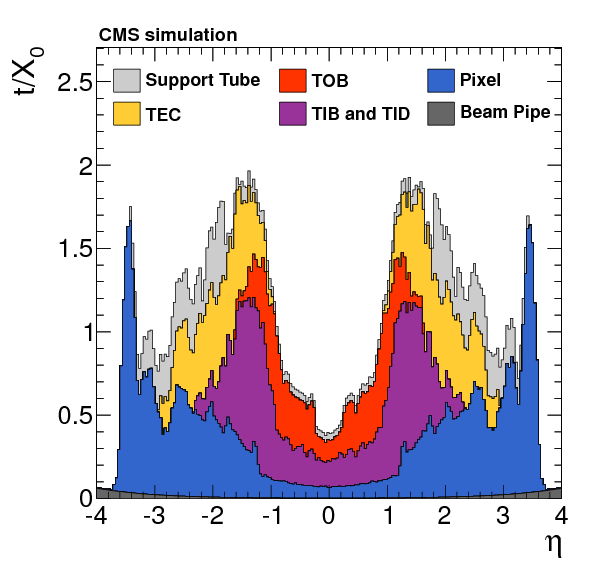
\includegraphics[width=\textwidth]{figures/tracker_material_budget.png}
    \caption{
        The thickness of material, $t$, divided by the radiation length,
        \radiationlength, encountered by particles leaving the nominal
        interaction point before reaching ECAL.
    }
    \label{fig:tracker_material}
\end{figure}

The reconstruction of electrons with $\pt > 20 \GeV$ in CMS starts with an
electron-like cluster of energy in ECAL \cite{eg_reco_2010}. In order to
account for energy lost to bremsstrahlung photons, additional clusters at
constant $\eta$ but changing $\phi$ are added together to form superclusters
\cite{baffioni_2007}.

From these superclusters, a point on the tracker where the electron is likely
to have come from is determined by propagating the energy weighted mean
position of the supercluster back through the magnetic field. This spot is then
used to seed  track finding algorithm in the pixel layer. Hits in the tracker
are searched from starting at the innermost layer and working outward. In order
to account for the changing track shape of the track as the electron loses
energy from interacting with the tracker material, a ``Gaussian Sum Filter''
(GSF) is used \cite{adam_2005}. Low energy electrons ($\ET < 15 \GeV$) are
constructed with \pt from the tracker and \ET from ECAL, but for electrons with
higher energy the ECAL energy alone is used to avoid issues introduced by
possible poor fits in the tracker. The $\eta$ and $\phi$ of all electron
candidates, regardless of energy, is taken from the track.

\section{Electron Variables}
\label{sec:electron_variables}

Reconstructed electrons have multiple variables that indicate their quality.
These variables are broken down into three main categories:

\begin{description}
    \item[Isolation:] \hfill \\
        These variables measures how much energy from other particles is
        deposited near the electron in the detector and are used to help reject
        jets.
    \item[Identification (ID):] \hfill \\
        These variables quantify how much like an electron the reconstructed
        particle looks like and are used to reject pions and other charged
        particles.
    \item[Conversion Rejection:] \hfill \\
        These variables are used to reject electrons from \photontoee
        conversions.
\end{description}

\subsection{Isolation}

Hadronic jets sometimes produce electrons in the numerous decays happening
within them. These electrons can be rejected by looking at the sum of the
energy in the tacker, ECAL, and HCAL around the electron, as electrons in jets
will have a large amount of energy surrounding them, whereas electrons from \Z
decays will tend to be isolated.

The isolations used in the trigger (\SingleElectronTrigger) are defined as
follows:

\begin{equation}
    \HCALISO = \DeltaRSum \ETHCAL
\end{equation}

\begin{equation}
    \ECALISO = \DeltaRSum \ETECAL - \ETSC
\end{equation}

Where \DeltaRSum is a sum on the energy in a $\Delta R < 0.3$ cone around the
supercluster location, \ETHCAL is the energy in HCAL, \ETECAL is the energy in
ECAL, and \ETSC is the energy of the supercluster, which is subtracted out of
the ECAL isolation sum. No subtraction is applied to the HCAL isolation as we
expect all of the electron's energy to be contained in ECAL.

Offline different isolation variables are defined that are more expensive to
compute. This isolation uses \particleflow\cite{particle_flow_2010} and
computes a single isolation number by combining the tracker, ECAL, and HCAL.
\ParticleFlow is a method of reconstructing jets that uses information for
every subdetector and tries to reconstruct the individual particles in a jet by
matching them to their responses in the various subdetectors. To keep the
algorithm simple, \particleflow categorizes every particle into one of four
types: photons, electrons, muons, and pions. A photon is a particle with energy
only deposited in ECAL. An electron is a particle with an ECAL energy deposit
and a track. A muon is a track in the central tracker matched to a track in the
muon system. A pion is any energy cluster in HCAL with a matching ECAL cluster
and track. These particle flow jets are used to calculate an energy per area
due to pileup, $\rho$, in the detector which is used to remove the pileup
contribution from the isolation sum. The \particleflow isolation, $\PFISO$, is
given by:

\begin{equation}
    \PFISO = \DeltaRSum \left(\ptTrack + \ETECAL + \ETHCAL\right) - \ptElectron
    - \ETSC - 0.3^{2} \pi \rho
\end{equation}

Where the variables are the same as above, with the addition of \ptTrack, which
is the \pt of all tracks in the tracker, \ptElectron, which is the \pt of the
electron's track, and $\left(0.3^{2} \pi \rho\right)$, which is the energy from
pileup in a cone of $\Delta R < 0.3$ around the electron.

\subsection{Identification}

The shape of the electromagnetic shower in the calorimeters is used to
discriminate between electrons and other particles. Electrons generally have
very narrow showers whereas hadronic particles have wide showers. The size of
the shower in $\eta$ is given by \sigmaietaieta. Electron showers are mostly
contained within ECAL and so the ratio of energy around the hit in HCAL over
the energy around the hit in ECAL, \HOverE, is also used to parameterize the
shower shape.

The matching of the track with the supercluster in \coordetaphi space is given
by \dphiin and \detain.  The compatibility of energy of the supercluster and
the momentum of the track is given by \ooeoop. Using these variables photons
can be rejected as they interact in ECAL but leave no track in the tracker.

\subsection{Conversion Rejection}

Conversions generally happen away from the vertex and so the distances of the
hits in the track from the vertex are useful quantities to reject conversions.
The transversal and longitudinal separation between the track and the primary
vertex are given by $d_{0}$ and $d_{z}$. Conversions generally happen deep in
the tracker and so tracks from them will have missing layers, given by \nmiss.
Conversions also have low vertex fit probability, \pvtx, indicating that their
track likely did not come from the primary vertex.

\section{Energy Corrections}
\TODO{Shervin's Regression}
